
\begin{document}

\chapter{Testing}

\label{chapter:testing}

The correctness of the tracking system is verified by seeing whether multiple skeletons of the same person are matched correctly in different interaction scenarios. The researcher is interested in whether the application has accomplished the following tasks, as well as the objectives listed Chapter~\ref{chapter:objectives}.

\begin{enumerate}
  \item The skeletons from different Kinect fields of view are matched to the correct person in the scene.
  \item There is a small difference between the multiple skeletons of the same person after transformed into the same perspective.
  \item The skeletons can be transformed into different Kinects' coordinate system.
  \item The system shows persistent tracking when the user moves about in the same environment.
\end{enumerate}

The main goal of the project is to demonstrate persistent tracking results in occluded environments and scenarios involving complex human interactions. Figure~\ref{fig:tracking_disjoined_views} shows that the current system can track a person from a distance. When the person is out of the viewing range, the system will show immediate feedback to the users (See Figure~\ref{fig:tracking_confused}). The tracking system will recover the skeletons when the person reappears.

\begin{figure}[!h]
  \centering
  
  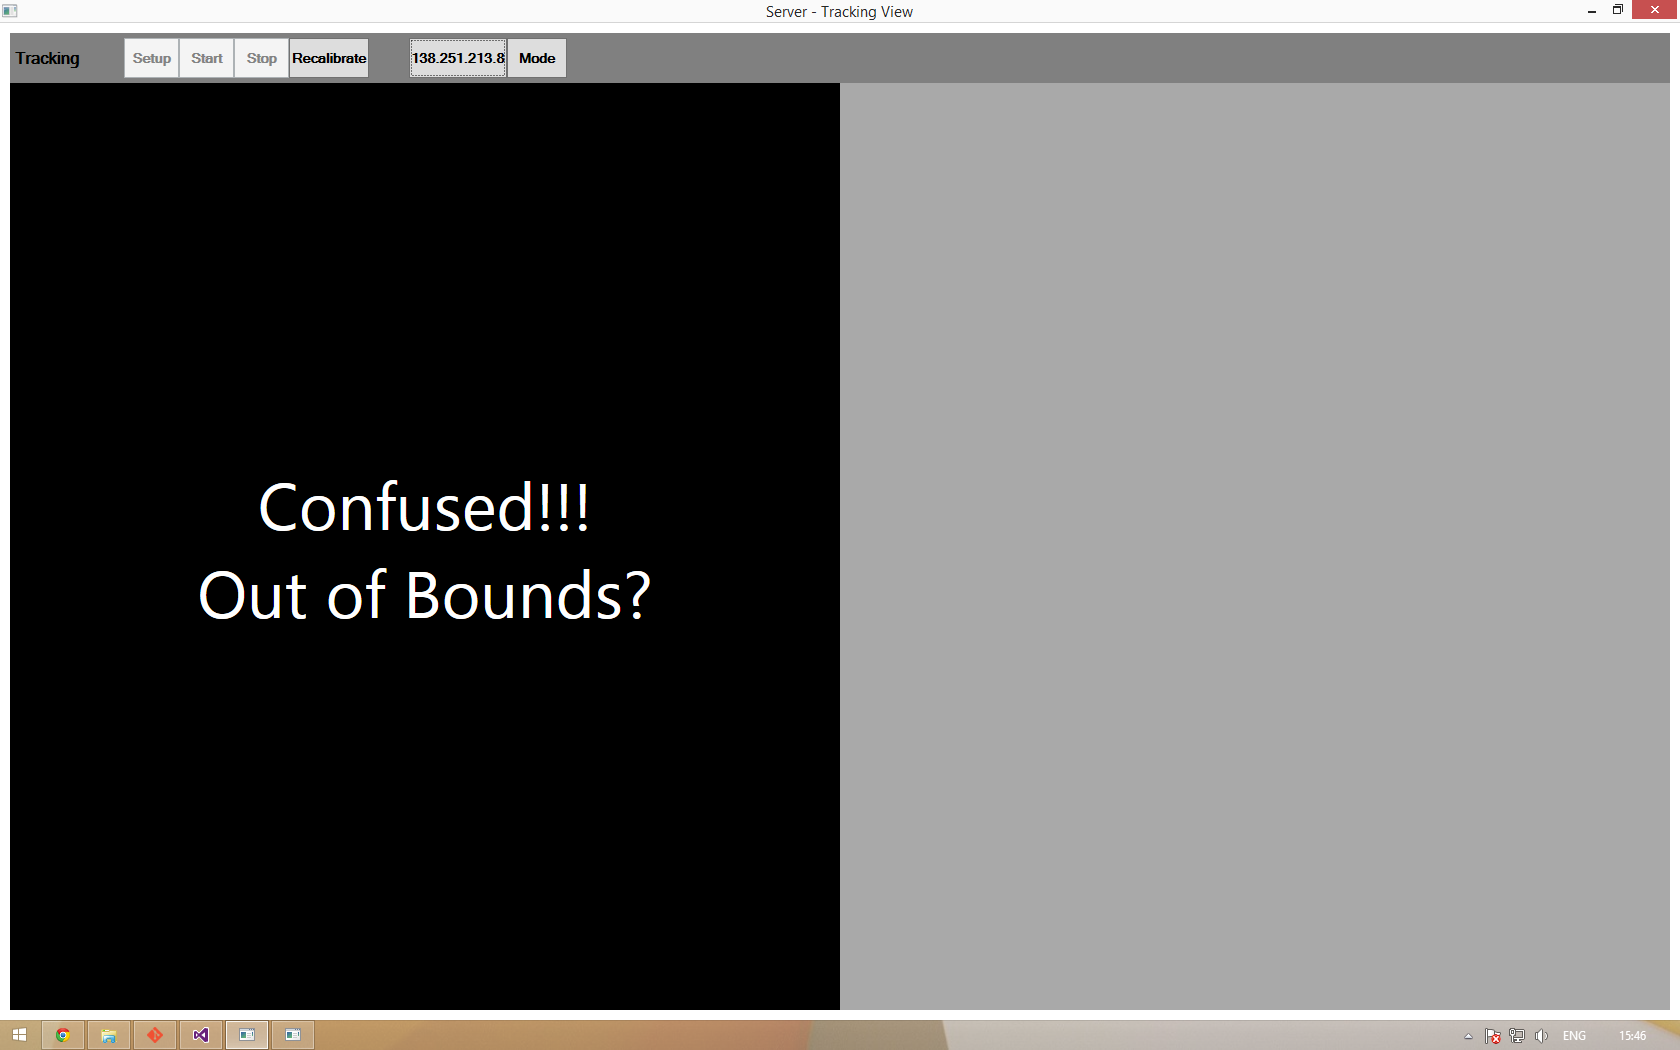
\includegraphics[width=0.5\linewidth]{figs/confused}

  \caption{User interface showing a reminder when the tracker detects people have disappeared.}
  
  \label{fig:tracking_confused}
\end{figure}

The current system resolves occlusion by combining joint information from multiple cameras. Figure~\ref{fig:occlusion_fill_in_gaps} demonstrates that the system can fuse fuse joint information seamlessly. The person is self-occluded if he stands in a position such that one Kinect cannot fully see all the joints, but two Kinects combined can have a complete view of the person. The researcher turns his body away from the primary Kinect, showing his right arm only to the second Kinect. The system constructs the average skeleton with joints that maximize the confidence level about the spatial information of the person. More results will discussed in Chapter~\ref{chapter:studies} and Chapter~\ref{chapter:results}.

\begin{figure}[!h]
  \centering
  \subfloat[An instance where the person is visible to both Kinects]{
    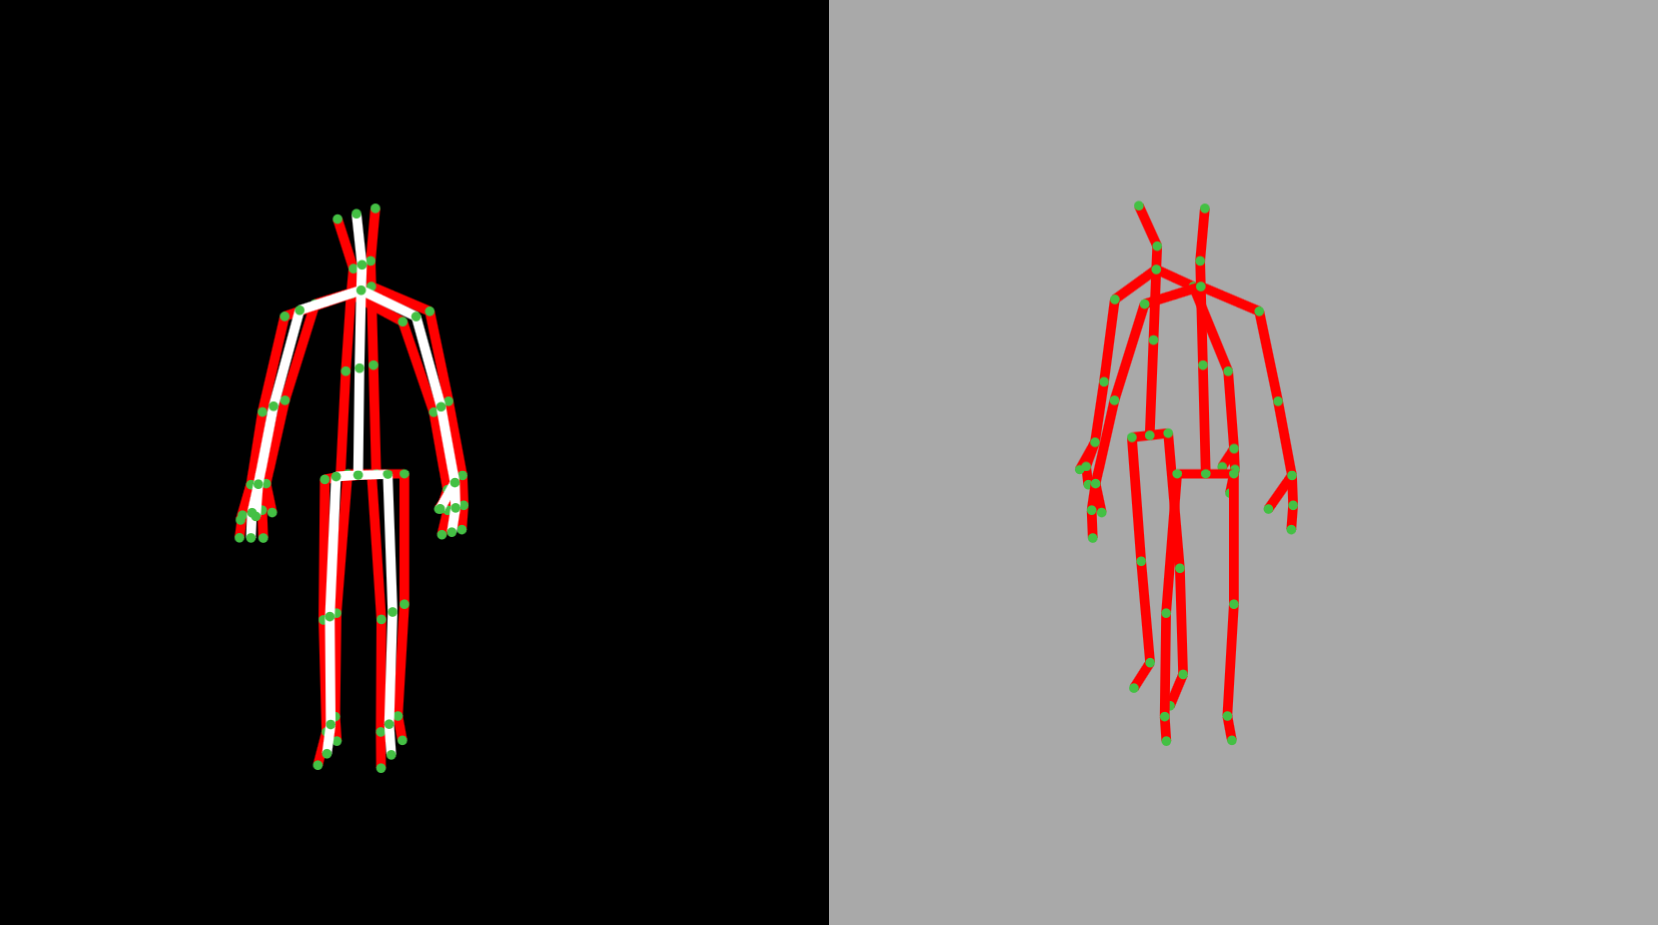
\includegraphics[width=0.5\linewidth]{figs/fill_in_gaps_before}
  }
  \subfloat[An instance where when the person is self-occluded, and the system creates the average skeleton using the joints that have the highest confidence level]{
    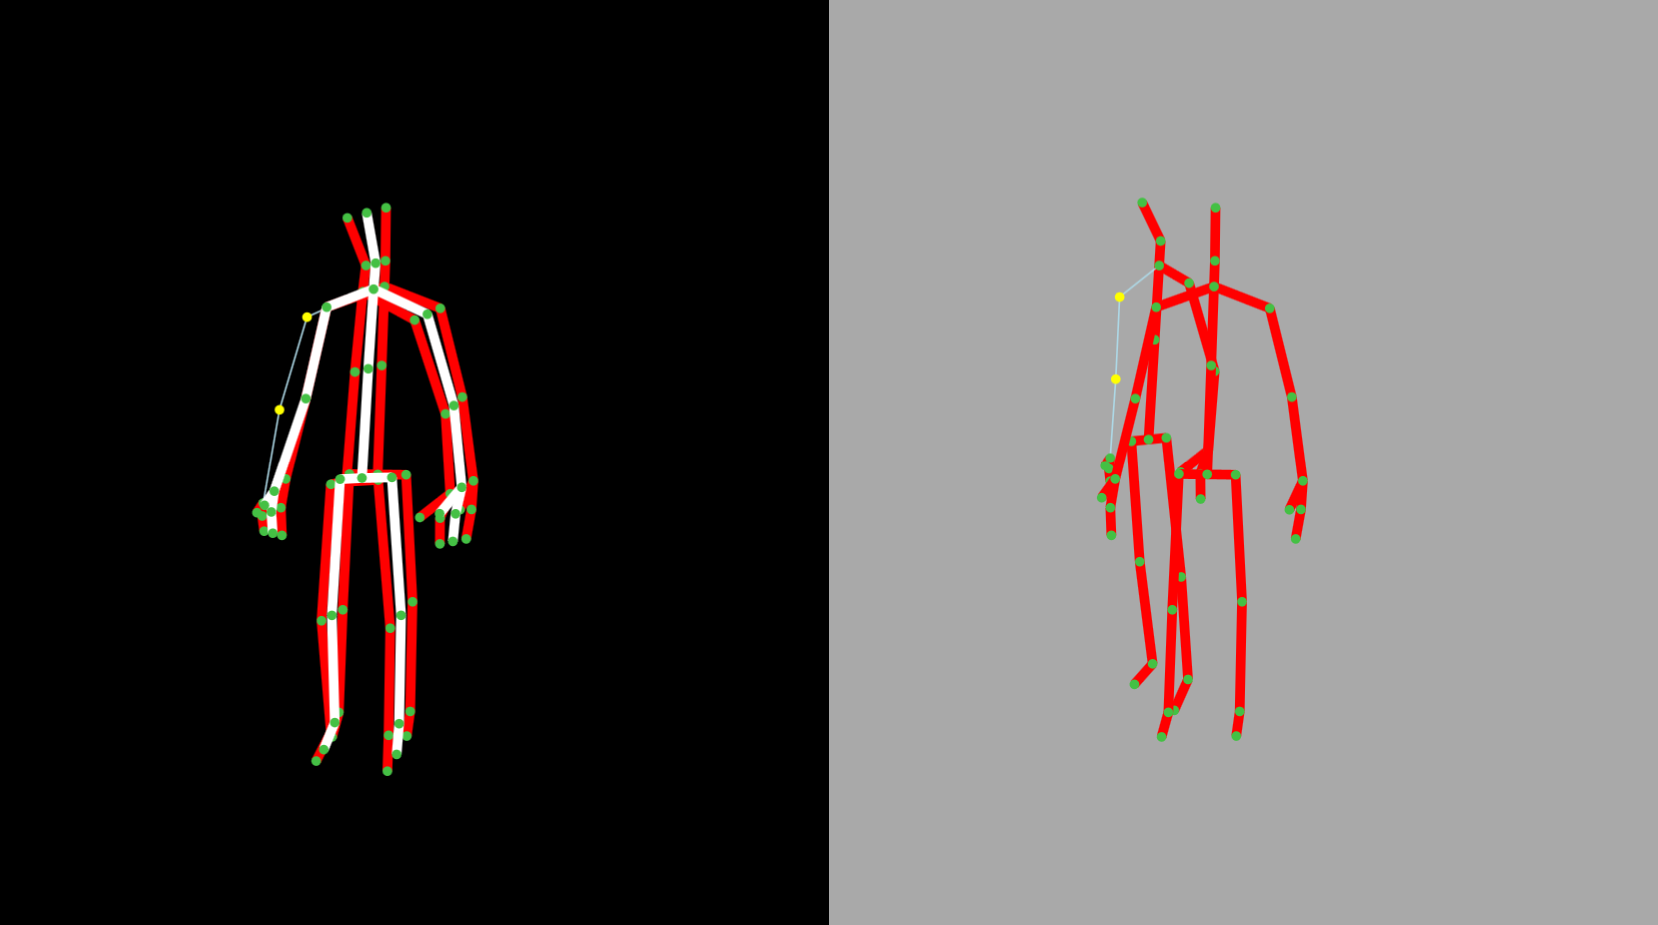
\includegraphics[width=0.5\linewidth]{figs/fill_in_gaps_after}
  }

  \caption{The average skeleton reconstructed leveraging information about actively tracked joints from multiple Kinects}
  
  \label{fig:occlusion_fill_in_gaps}
\end{figure}

\end{document}
